\documentclass[tikz, border=3pt]{standalone}

\usepackage{amsmath,amssymb}
\usepackage{pgfplots}
\pgfplotsset{compat=1.18}
\usepgfplotslibrary{groupplots}
\usetikzlibrary{arrows.meta}
\usepackage{xcolor}

\definecolor{utnblue}{RGB}{0, 51, 102}
\definecolor{utnred}{RGB}{204, 0, 0}

% Eje horizontal en unidades de 10^3 pi rad/s
\pgfplotsset{
    espectro/.style={
        axis lines=middle,
        width=13cm, height=4.6cm,
        xmin=-24, xmax=24,
        ymin=-500, ymax=6200,
        ytick={2500,5000},
        yticklabels={$2500$,$5000$},
        tick label style={font=\tiny},
        label style={font=\scriptsize},
        title style={font=\scriptsize, at={(axis description cs:1,1)},
                     anchor=north east, xshift=-2pt, yshift=-2pt},
        xticklabel style={fill=white, inner sep=1.5pt},
        every axis x label/.style={at={(ticklabel* cs:1)}, anchor=west},
        every axis y label/.style={at={(ticklabel* cs:1)}, anchor=south},
        enlargelimits=false,
        clip mode=individual,
        axis on top,
        xlabel={$\omega$},
        ylabel={$X_s(j\omega)$},
    },
}

\begin{document}
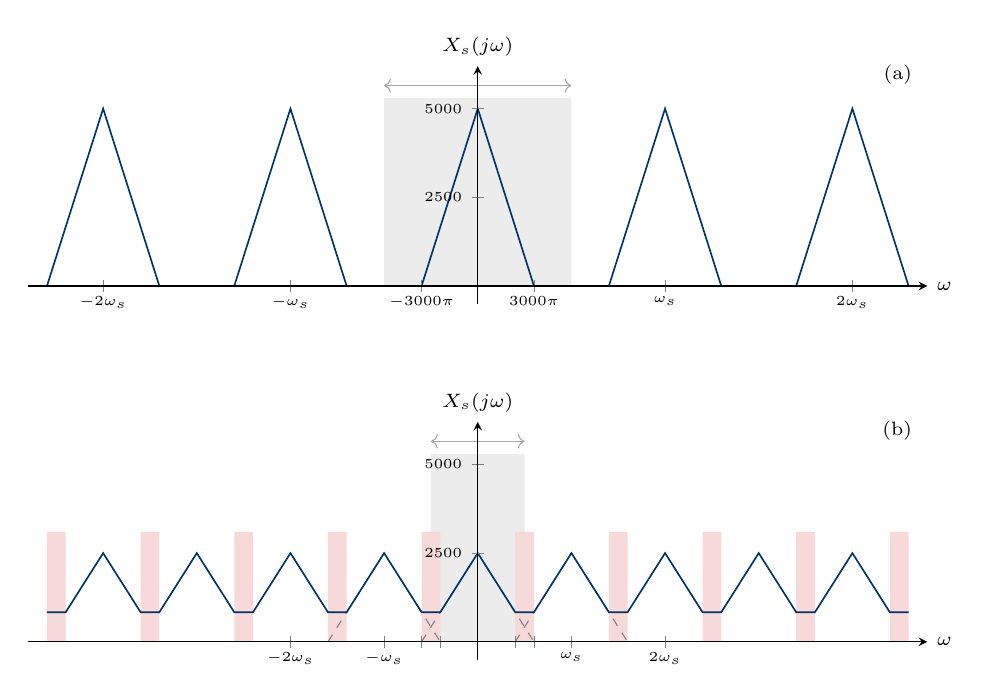
\begin{tikzpicture}[font=\scriptsize]

\begin{groupplot}[
    group style={group size=1 by 2, vertical sep=1.5cm},
    espectro,
]

% =========== (a) Delta t = 0,2 ms : omega_s = 10000 pi ===========
\nextgroupplot[title={(a)},
    xtick={-20,-10,-3,3,10,20},
    xticklabels={$-2\omega_s$,$-\omega_s$,$-3000\pi$,$3000\pi$,$\omega_s$,$2\omega_s$},
]
\addplot[draw=none, fill=gray!15] coordinates {(-5,0) (5,0) (5,5300) (-5,5300)} \closedcycle;
\draw[gray!70, <->] (axis cs:-5,5650) -- (axis cs:5,5650);
\addplot[utnblue, semithick] coordinates {(-23,0) (-20,5000) (-17,0)};
\addplot[utnblue, semithick] coordinates {(-13,0) (-10,5000) (-7,0)};
\addplot[utnblue, semithick] coordinates {(-3,0)  (0,5000)   (3,0)};
\addplot[utnblue, semithick] coordinates {(7,0)   (10,5000)  (13,0)};
\addplot[utnblue, semithick] coordinates {(17,0)  (20,5000)  (23,0)};

% =========== (b) Delta t = 0,4 ms : omega_s = 5000 pi ===========
\nextgroupplot[title={(b)},
    xtick={-10,-5,-3,-2,2,3,5,10},
    xticklabels={$-2\omega_s$,$-\omega_s$,,,,,$\omega_s$,$2\omega_s$},
]
\addplot[draw=none, fill=gray!15] coordinates {(-2.5,0) (2.5,0) (2.5,5300) (-2.5,5300)} \closedcycle;
\draw[gray!70, <->] (axis cs:-2.5,5650) -- (axis cs:2.5,5650);

% zonas de solapamiento (una por cada par de copias vecinas)
\addplot[draw=none, fill=utnred!15] coordinates {(2,0) (3,0) (3,3100) (2,3100)} \closedcycle;
\addplot[draw=none, fill=utnred!15] coordinates {(-3,0) (-2,0) (-2,3100) (-3,3100)} \closedcycle;
\addplot[draw=none, fill=utnred!15] coordinates {(7,0) (8,0) (8,3100) (7,3100)} \closedcycle;
\addplot[draw=none, fill=utnred!15] coordinates {(-8,0) (-7,0) (-7,3100) (-8,3100)} \closedcycle;
\addplot[draw=none, fill=utnred!15] coordinates {(12,0) (13,0) (13,3100) (12,3100)} \closedcycle;
\addplot[draw=none, fill=utnred!15] coordinates {(-13,0) (-12,0) (-12,3100) (-13,3100)} \closedcycle;
\addplot[draw=none, fill=utnred!15] coordinates {(17,0) (18,0) (18,3100) (17,3100)} \closedcycle;
\addplot[draw=none, fill=utnred!15] coordinates {(-18,0) (-17,0) (-17,3100) (-18,3100)} \closedcycle;
\addplot[draw=none, fill=utnred!15] coordinates {(22,0) (23,0) (23,3100) (22,3100)} \closedcycle;
\addplot[draw=none, fill=utnred!15] coordinates {(-23,0) (-22,0) (-22,3100) (-23,3100)} \closedcycle;

% copias individuales
\addplot[gray, dashed, thin] coordinates {(-8,0) (-5,2500) (-2,0)};
\addplot[gray, dashed, thin] coordinates {(-3,0) (0,2500)  (3,0)};
\addplot[gray, dashed, thin] coordinates {(2,0)  (5,2500)  (8,0)};

% suma de todas las copias
\addplot[utnblue, semithick] coordinates {
    (-23,833) (-22,833) (-20,2500) (-18,833) (-17,833) (-15,2500)
    (-13,833) (-12,833) (-10,2500) (-8,833)  (-7,833)  (-5,2500)
    (-3,833)  (-2,833)  (0,2500)   (2,833)   (3,833)   (5,2500)
    (7,833)   (8,833)   (10,2500)  (12,833)  (13,833)  (15,2500)
    (17,833)  (18,833)  (20,2500)  (22,833)  (23,833)
};

\end{groupplot}

\end{tikzpicture}
\end{document}
